\subsection{Tile set}
\label{gadgets}


% { \tt Gadget}( $\left\langle \text{Input} \right\rangle, \left\langle \text{Output}  \right\rangle$ )

\newcommand{\warpunit}{{\tt Warp\_Unit}}
\newcommand{\prewarp}{{\tt Pre\_Warp}}
\newcommand{\firstwarp}{{\tt First\_Warp}}
\newcommand{\warpbridge}{{\tt Warp\_Bridge}}
\newcommand{\secondwarp}{{\tt Second\_Warp}}
\newcommand{\postwarp}{{\tt Post\_Warp}}

\newcommand{\dtop}{{\tt Digit\_Top}}
\newcommand{\dwriter}{{\tt Digit\_Writer}}
\newcommand{\dreader}{{\tt Digit\_Reader}}

\newcommand{\returnfromdonereadnextrow}{{\tt Return\_From\_Digit1\_Read\_Next\_Row}}
\newcommand{\returnfromdtworeadnextrow}{{\tt Return\_From\_Digit2\_Read\_Next\_Row}}
\newcommand{\returnfromdthreereadnextrow}{{\tt Return\_From\_Digit3\_Read\_Next\_Row}}

\newcommand{\returnfromdonereaddtwo}{{\tt Return\_From\_Digit1\_Read\_Digit2}}
\newcommand{\returnfromdonereaddtwocasetwo}{{\tt Return\_From\_Digit1\_Read\_Digit2\_Case2}}
\newcommand{\returnfromdtworeaddthree}{{\tt Return\_From\_Digit2\_Read\_Digit3}}
\newcommand{\returnfromdthreereaddone}{{\tt Return\_From\_Digit3\_Read\_Digit1}}

\newcommand{\inc}{{\tt op}}

\newcommand{\dtopdonecaseone}{{\tt Digit\_Top\_Digit1\_Case1}}
\newcommand{\dtopdonecasetwo}{{\tt Digit\_Top\_Digit1\_Case2}}
\newcommand{\dtopdtwocasetwo}{{\tt Digit\_Top\_Digit2\_Case2}}
\newcommand{\dtopcasethree}{{\tt Digit\_Top\_Case3}}

\newcommand{\gadgetref}{from the general gadget shown in Figure~}
\newcommand{\mgadgetref}{from the micro-gadget shown in Figure~}

% todo: fix wording
When describing a special case, i.e. ``digit $x$ -- case $y$'', whatever follows
will only apply to the MSR (due to each case only affecting the MSR.)

\subsubsection{ Line Gadgets }

\begin{figure}[H]
    \centering
    \begin{subfigure}[t]{0.15\textwidth}
        \centering
        \includegraphics[width=0.15\textwidth]{south_to_north_line}
        \caption{\label{fig:north_line} {\tt Line\_North}}
    \end{subfigure}%
    ~
    \begin{subfigure}[t]{0.15\textwidth}
        \centering
        \includegraphics[width=0.15\textwidth]{north_to_south_line}
        \caption{\label{fig:south_line} {\tt Line\_South} }
    \end{subfigure}%
    ~
    \caption{\label{fig:line_gadgets} {\tt Line} gadgets}
\end{figure}

We will use the notation {\tt LineN\_North} and {\tt LineN\_South} where {\tt N} corresponds to the length of a specific line gadget.


\subsection{Initial Value (updated to assemble right to left like the other gadgets)}
    We begin by encoding $\mathcal{C}_0$ with the Seed unit. It has $\ceil*{\frac{d}{3}}$ digit regions.
    Each digit region has three digits, except for the most significant digit region (MSR) which has $d \mod 3$
    if $d \mod 3 \not= 0$, otherwise it has 3 digits.


    \begin{figure}[H]
        \centering
        \begin{subfigure}[t]{0.3\textwidth}
            \centering
            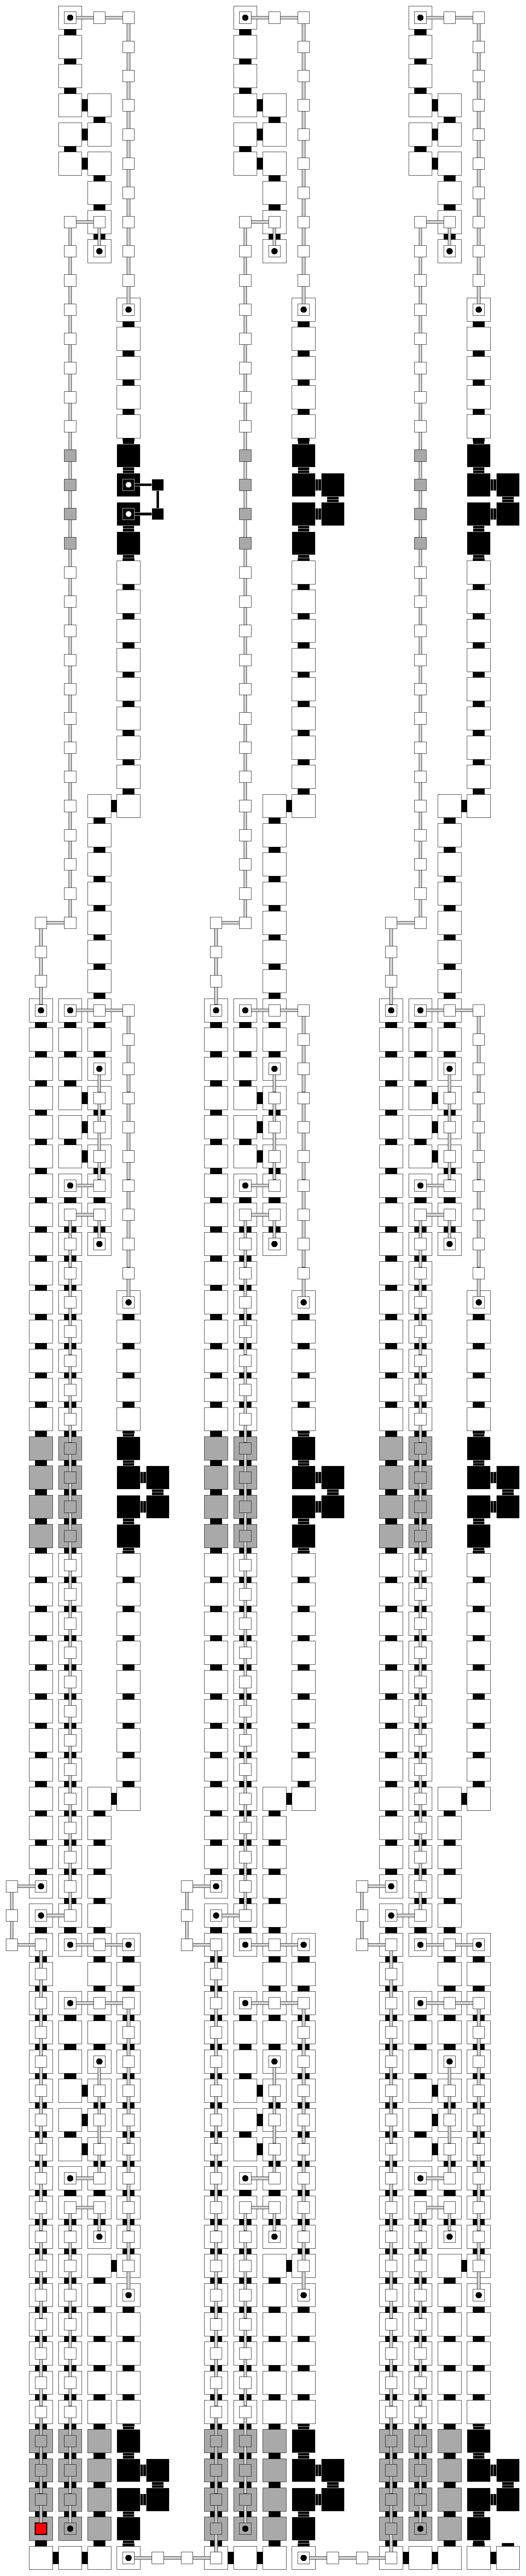
\includegraphics[width=0.3\textwidth]{seed/seed_overview_case3}
            \caption{\label{fig:initial_value_case3} Initial value case 3}
        \end{subfigure}%
        ~
        \begin{subfigure}[t]{0.3\textwidth}
            \centering
            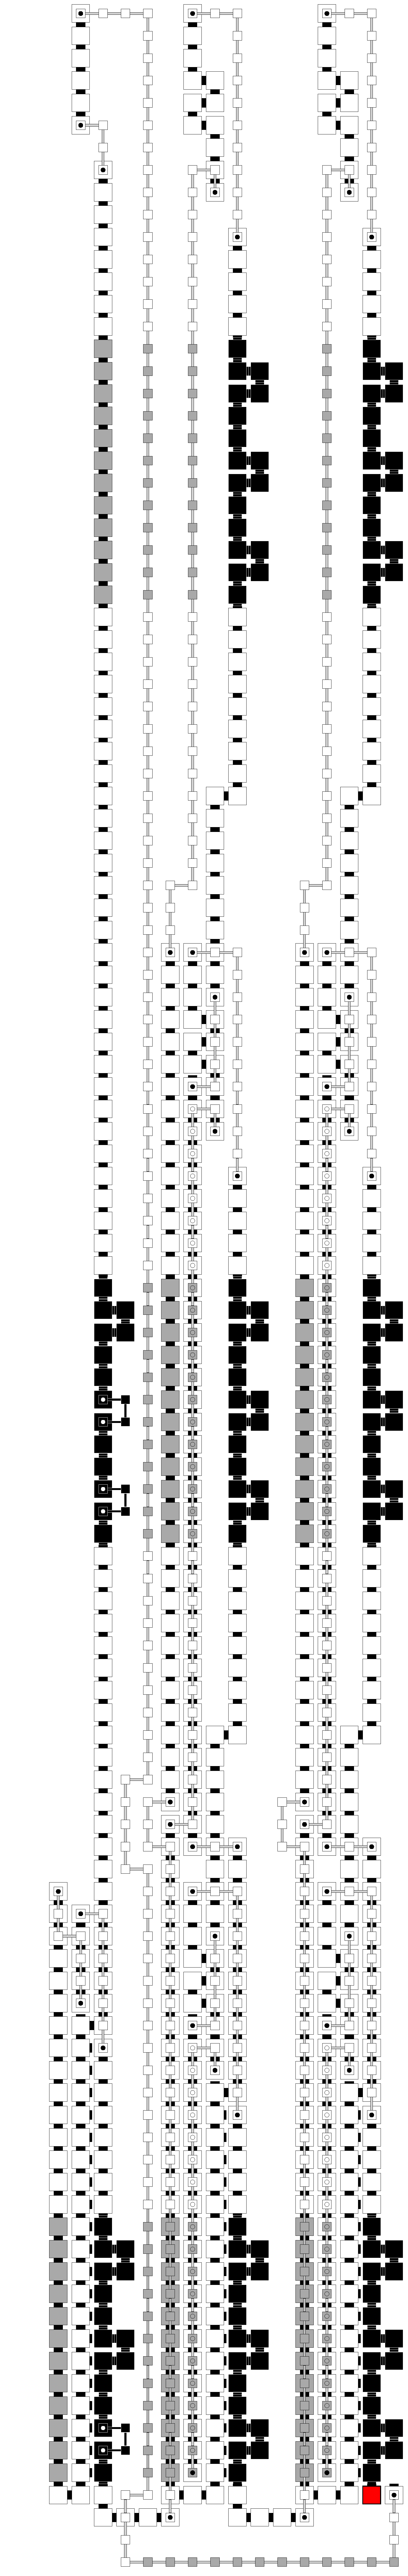
\includegraphics[width=0.3\textwidth]{seed/seed_overview_case2}
            \caption{\label{fig:initial_value_case2} Initial value case 2}
        \end{subfigure}%
        ~
        \begin{subfigure}[t]{0.3\textwidth}
            \centering
            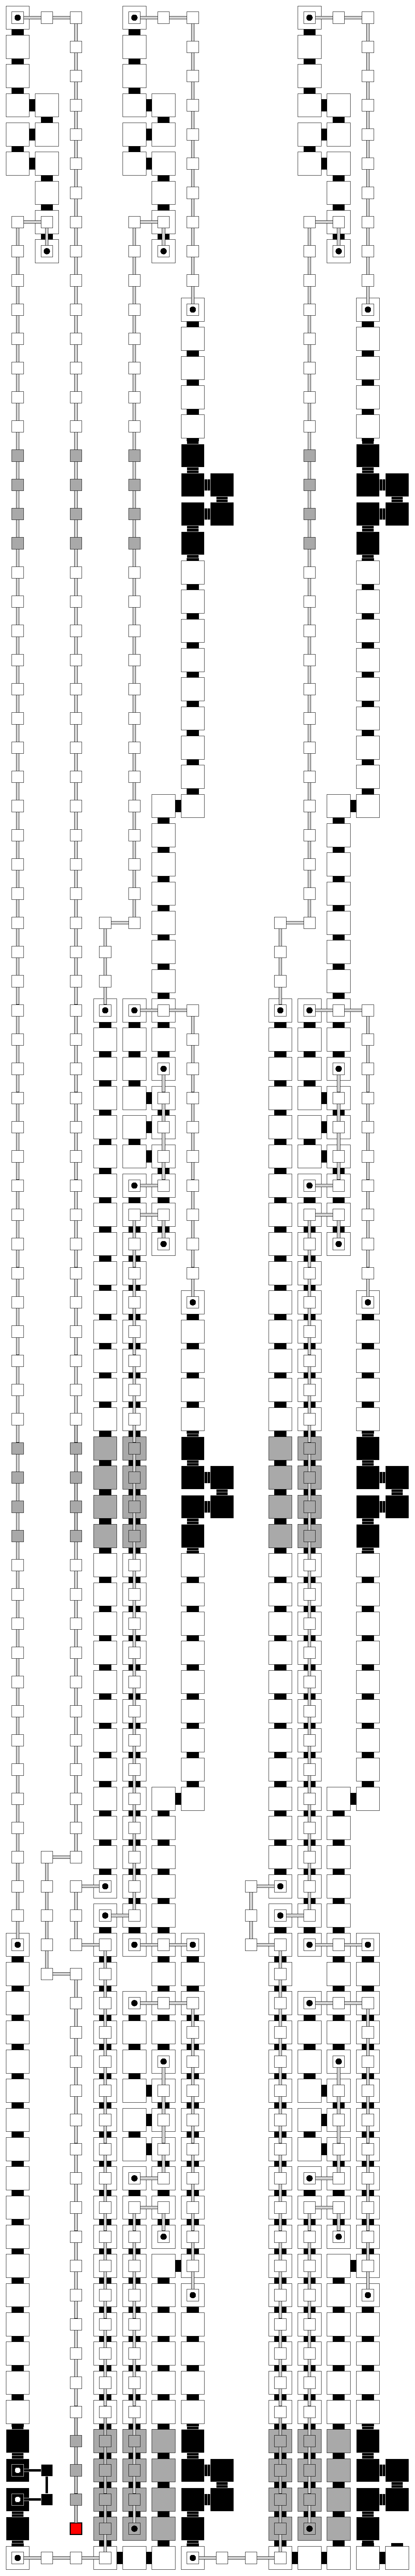
\includegraphics[width=0.3\textwidth]{seed/seed_overview_case1}
            \caption{\label{fig:initial_value_case1} Initial value case 1}
        \end{subfigure}%
        ~
    \end{figure}

    For each $i=0,\ldots,d$

    \begin{itemize}
        \item Create
        $\begin{aligned}[t]
            {\tt Seed\_Start}(&\left\langle {\tt DigitWriter}, {\tt Seed}, i, \inc \right\rangle \; )
        \end{aligned}$

        \item {\tt Digit}: For each $j=0,\ldots,l$ and each $b$ in $bin(C_0[i])[j]$:
        \begin{itemize}
            \item if $j = 0$: create
            $\begin{aligned}[t]
                \dwriter(&\left\langle {\tt Digit\_1} \right\rangle, \left\langle {\tt Seed\_Bit}, i, j + 1 \right\rangle \;)
            \end{aligned}$ from the general gadget shown in Figure~\ref{fig:write_0} if $b = 0$ or Figure~\ref{fig:write_1} if $b = 1$.

            \item if $0 \leqslant j \leqslant l$: create
            $\begin{aligned}[t]
                \dwriter(&\left\langle {\tt Seed\_Bit}, i, j \right\rangle, \left\langle {\tt Seed\_Bit}, i, j + 1 \right\rangle \;)
            \end{aligned}$ from the general gadget shown in Figure~\ref{fig:write_0} if $b = 0$ or Figure~\ref{fig:write_1} if $b = 1$.

            \item if $j = l$:
            $\begin{aligned}[t]
                \dwriter(&\left\langle {\tt Seed\_Bit}, i, j \right\rangle, \left\langle {\tt Seed\_DigitTop\_1}, i \right\rangle \;)
            \end{aligned}$ from the general gadget shown in Figure~\ref{fig:write_0} if $b = 0$ or Figure~\ref{fig:write_1} if $b = 1$.

        \end{itemize}

        \item {\dtop}: The following statements create the gadget shown in Figure~\ref{fig:digit_top_general}
        \begin{itemize}
            \item Create
            $\begin{aligned}[t]
                {\tt North\_Line5}(& \left \langle {\tt Seed\_DigitTop\_1},    i \right\rangle,
                                     \left \langle {\tt Seed\_DigitTop\_1\_A}, i \right\rangle \;)
            \end{aligned}$ from the micro-gadget\\shown in Figure~\ref{fig:north_line}

            \item Create
            $\begin{aligned}[t]
                {\tt Topper}(& \left \langle {\tt DigitTop\_1\_A}, i \right\rangle,
                               \left \langle {\tt DigitTop\_1\_B}, i \right\rangle \;)
            \end{aligned}$ from the micro-gadget shown in\\ Figure~\ref{fig:topper_gen}

            \item Create
            $\begin{aligned}[t]
                {\tt South\_Line4\textit{l}}(& \left \langle {\tt DigitTop\_1\_B}, i \right\rangle,
                                               \left \langle {\tt ReturnD3ReadD1}, i \right\rangle \;)
            \end{aligned}$ from the\\micro-gadget shown in Figure~\ref{fig:south_line}
        \end{itemize}




        \item Create
        $\begin{aligned}[t]
            \returnfromdonereaddtwo(&\left\langle {\tt TODO} \right\rangle,
                                     \left\langle {\tt TODO} \right\rangle \;)
        \end{aligned}$

        \item Create
        $\begin{aligned}[t]
            Single tile(&\left\langle {\tt TODO} \right\rangle,
                         \left\langle {\tt TODO} \right\rangle \;)
        \end{aligned}$

        \item Create
        $\begin{aligned}[t]
            \secondwarp(&\left\langle {\tt TODO} \right\rangle,
                         \left\langle {\tt TODO} \right\rangle \;)
        \end{aligned}$

        \item Create
        $\begin{aligned}[t]
            \postwarp(&\left\langle {\tt TODO} \right\rangle,
                       \left\langle {\tt TODO} \right\rangle \;)
        \end{aligned}$

        \item Create
        $\begin{aligned}[t]
            \dwriter(&\left\langle {\tt TODO} \right\rangle,
                      \left\langle {\tt TODO} \right\rangle \;)
        \end{aligned}$

        \item Create
        $\begin{aligned}[t]
            \dtop(&\left\langle {\tt TODO} \right\rangle,
                   \left\langle {\tt TODO} \right\rangle \;)
        \end{aligned}$

        \item Create
        $\begin{aligned}[t]
            \returnfromdtworeaddthree (&\left\langle {\tt TODO} \right\rangle,
                                        \left\langle {\tt TODO} \right\rangle \;)
        \end{aligned}$

        \item Create
        $\begin{aligned}[t]
            {\tt Three\_Digit\_Region\_Connector} (&\left\langle {\tt TODO} \right\rangle,
                                                    \left\langle {\tt TODO} \right\rangle \;)
        \end{aligned}$

        \item Create
        $\begin{aligned}[t]
            \firstwarp(&\left\langle {\tt TODO} \right\rangle,
                        \left\langle {\tt TODO} \right\rangle \;)
        \end{aligned}$

        \item Create
        $\begin{aligned}[t]
            \warpbridge(&\left\langle {\tt TODO} \right\rangle,
                         \left\langle {\tt TODO} \right\rangle \;)
        \end{aligned}$

        \item Create
        $\begin{aligned}[t]
            \secondwarp(&\left\langle {\tt TODO} \right\rangle,
                         \left\langle {\tt TODO} \right\rangle \;)
        \end{aligned}$

        \item Create
        $\begin{aligned}[t]
            \postwarp(&\left\langle {\tt TODO} \right\rangle,
                       \left\langle {\tt TODO} \right\rangle \;)
        \end{aligned}$

        \item Create
        $\begin{aligned}[t]
            \dwriter(&\left\langle {\tt TODO} \right\rangle,
                      \left\langle {\tt TODO} \right\rangle \;)
        \end{aligned}$

        \item Create
        $\begin{aligned}[t]
            \dtop(&\left\langle {\tt TODO} \right\rangle,
                   \left\langle {\tt TODO} \right\rangle \;)
        \end{aligned}$

        \item Create
        $\begin{aligned}[t]
            \returnfromdthreereadnextrow(&\left\langle {\tt TODO} \right\rangle,
                                          \left\langle {\tt TODO} \right\rangle \;)
        \end{aligned}$

        \item Create
        $\begin{aligned}[t]
            {\tt Digit\_Region\_Bridge}(&\left\langle {\tt TODO} \right\rangle,
                                         \left\langle {\tt TODO} \right\rangle \;)
        \end{aligned}$
    \end{itemize}


\subsection{ Counter Unit }

    \subsubsection{ Digit readers }

\begin{itemize}

\item For each $i = 1,2,3$,
                   $j = l-1,\ldots,1$,
                   $u \in \{0, 1\}^j$, and
                   $\inc \in \{{\tt increment}, {\tt copy} \}$:
    \begin{itemize}
        \item if $j = 0$:
        Create
        $\begin{aligned}[t]
            \dreader(& \left\langle {\tt DigitReader}, i, \lambda, \inc \right\rangle, \\
                     & \left\langle {\tt DigitReader}, i, 0, \inc \right\rangle, \\
                     & \left\langle {\tt DigitReader}, i, 1, \inc \right\rangle \;)
        \end{aligned}$\\
        from the general gadget in Figure~\ref{fig:digit_read}

        \item if $1 \leqslant j \leqslant l -2$:
        Create
        $\begin{aligned}[t]
        \dreader(& \left\langle {\tt DigitReader}, i, u, \inc \right\rangle, \\
                 & \left\langle {\tt DigitReader}, i, 0u, \inc \right\rangle, \\
                 & \left\langle {\tt DigitReader}, i, 1u, \inc \right\rangle \;)
        \end{aligned}$\\
        from the general gadget in Figure~\ref{fig:digit_read}

        \item if $j = l - 1$:
        Create
        $\begin{aligned}[t]
            \dreader(& \left\langle {\tt DigitReader}, i, u, \inc \right\rangle, \\
                     & \left\langle {\tt PreWarp}, i, 0u, \inc \right\rangle, \\
                     & \left\langle {\tt PreWarp}, i, 1u, \inc \right\rangle \;)
        \end{aligned}$\\
        from the general gadget in Figure~\ref{fig:digit_read}

    \end{itemize}


\end{itemize}

\begin{figure}[H]
    \centering
    \begin{subfigure}[t]{0.2\textwidth}
        \centering
        \includegraphics[width=0.2\textwidth]{read/read_0}
        \caption{\label{fig:read_0} {\tt Counter\_Read\_0}}
    \end{subfigure}%
    ~
    \begin{subfigure}[t]{0.2\textwidth}
        \centering
        \includegraphics[width=0.2\textwidth]{read/read_1}
        \caption{\label{fig:read_1} {\tt Counter\_Read\_1}}
    \end{subfigure}%
    \caption{\label{fig:digit_read} {\tt {Counter\_Read}}}
\end{figure}

    % For each digit length L
\subsubsection{ Warping }

% For each index in 1, 2, 3, and carry in 0,1
    For each $i = 1, 2, 3$, $u \in \{0, 1\}^l$, and each $\inc \in \{ {\tt increment, copy } \}$
    (note: since this might not be the correct notation, in words: do this for each binary encoded digit of length $l$,
    for each digit-region index, and both copy/increment signals)


    \begin{itemize}

        \item if $u$ ends with 00:
        Create
        $\begin{aligned}[t]
            \prewarp(& \left\langle {\tt PreWarp},   i, u, \inc \right\rangle,
                       \left\langle {\tt FirstWarp}, i, u, \inc \right\rangle \;)
        \end{aligned}$ %\\ % from the general gadget in Figure~\ref{fig:pre_warp_general}

        \item if $u$ ends with 01:
        Create
        $\begin{aligned}[t]
            \prewarp(& \left\langle {\tt PreWarp},   i, u, \inc \right\rangle,
                       \left\langle {\tt FirstWarp}, i, u, \inc, {\tt msr} \right\rangle \;)
        \end{aligned}$ % \\ % from the general gadget in Figure~\ref{fig:pre_warp_case2_digit1_msr}

        \item if $u$ ends with 11:
        Create
        $\begin{aligned}[t]
            \prewarp(& \left\langle {\tt PreWarp},   i, u, \inc \right\rangle,
                       \left\langle {\tt FirstWarp}, i, u, \inc, {\tt msr}, {\tt msd} \right\rangle \;)
        \end{aligned}$

        Depending on the number of digits in the MSR, the gadget created in this step will differ.
        If $i$ is 1 (case 1) use the general gadget in Figure~\ref{fig:pre_warp_case1_digit1_msr}.
        If $i$ is 2 (case 2) use the general gadget in Figure~\ref{fig:pre_warp_case2_digit2_msr}.
        If $i$ is 3 (case 3) use the general gadget in Figure~\ref{fig:pre_warp_general}.


        \vspace{.5cm}

        \begin{figure}[H]
            \begin{subfigure}[t]{0.2\textwidth}
                \centering
                \includegraphics[width=0.2\textwidth]{warping/pre_warp_general}
                \caption{\label{fig:pre_warp_general} General }
            \end{subfigure}%
            ~
            \begin{subfigure}[t]{0.2\textwidth}
                \centering
                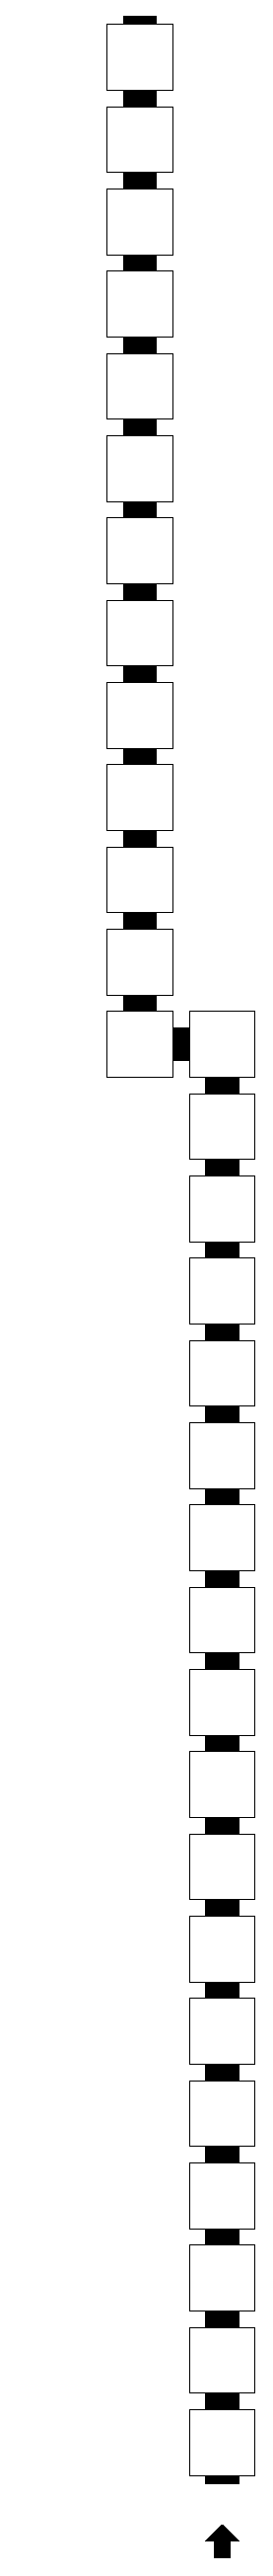
\includegraphics[width=0.2\textwidth]{warping/pre_warp_case1_digit1_msr}
                \caption{\label{fig:pre_warp_case1_digit1_msr} Digit 1 -- Case 1}
            \end{subfigure}%
            ~
            \begin{subfigure}[t]{0.2\textwidth}
                \centering
                \includegraphics[width=0.2\textwidth]{warping/pre_warp_case2_digit1_msr}
                \caption{\label{fig:pre_warp_case2_digit1_msr} Digit 1 -- Case 2}
            \end{subfigure}%
            ~
            \begin{subfigure}[t]{0.2\textwidth}
                \centering
                \includegraphics[width=0.2\textwidth]{warping/pre_warp_case2_digit2_msr}
                \caption{\label{fig:pre_warp_case2_digit2_msr} Digit 2 -- Case 2}
            \end{subfigure}%
            ~
            \caption{\label{fig:pre_warp_gadgets} {\prewarp} gadgets }
        \end{figure}


        \item A {\firstwarp} connects to a {\warpbridge} gadget in all cases except when it's assembling
              in the MSR and it is digit 1 in case 1 or 2, in which the {\firstwarp} gadget attaches directly
              to a {\postwarp}.

              \begin{itemize}
                \item if MSR has 1 digit and $u$ ends with 11: Create
                $\begin{aligned}[t]
                    \firstwarp(& \left\langle {\tt FirstWarp}, i, u, \inc \right\rangle, \\
                               & \left\langle {\tt FirstWarp}, i, u, \inc \right\rangle, \\
                               & \left\langle {\tt PostWarp},  i, u, \inc \right\rangle \;)
                \end{aligned}$
                \vspace{.5cm}


                \item if MSR has 2 digits and $u$ ends with 01: Create
                $\begin{aligned}[t]
                    \firstwarp(& \left\langle {\tt FirstWarp}, i, u, \inc \right\rangle, \\
                    & \left\langle {\tt FirstWarp},            i, u, \inc \right\rangle, \\
                    & \left\langle {\tt PostWarp},             i, u, \inc \right\rangle \;)
                \end{aligned}$
                \vspace{.5cm}


                \item if MSR has 2 digits and $u$ ends with 11: Create
                $\begin{aligned}[t]
                    \firstwarp(& \left\langle {\tt FirstWarp}, i, u, \inc \right\rangle, \\
                    & \left\langle {\tt FirstWarp},            i, u, \inc \right\rangle, \\
                    & \left\langle {\tt WarpBridge},           i, u, \inc \right\rangle \;)
                \end{aligned}$
                \vspace{.5cm}

                \item if MSR has 3 digits or $d$ starts with 00: Create
                $\begin{aligned}[t]
                    \firstwarp(& \left\langle {\tt FirstWarp},  i, u, \inc \right\rangle, \\
                               & \left\langle {\tt FirstWarp},  i, u, \inc \right\rangle, \\
                               & \left\langle {\tt WarpBridge}, i, u, \inc \right\rangle \;)
                \end{aligned}$

            \end{itemize}
        \vspace{.5cm}

        \item A {\warpbridge} gadget binds the last tile of the {\firstwarp} gadgets to the
             first tile of the {\secondwarp} gadgets. For digit 1 in cases 1 and 2, the
             {\warpbridge} is omitted from the {\warpunit}.

        \begin{itemize}
            \item Create
            $\begin{aligned}[t]
                \warpbridge(& \left\langle {\tt WarpBridge}, i, u, \inc \right\rangle, \\
                            & \left\langle {\tt SecondWarp}, i, u, \inc \right\rangle \;)
            \end{aligned}$
            \vspace{.5cm}
        \end{itemize}

        \begin{figure}[H]
            \centering
            \begin{subfigure}[t]{0.2\textwidth}
                \centering
                \includegraphics[width=0.2\textwidth]{warping/warp_bridge_general}
                \caption{\label{fig:warp_bridge_general} General}
            \end{subfigure}%
            ~
            \begin{subfigure}[t]{0.2\textwidth}
                \centering
                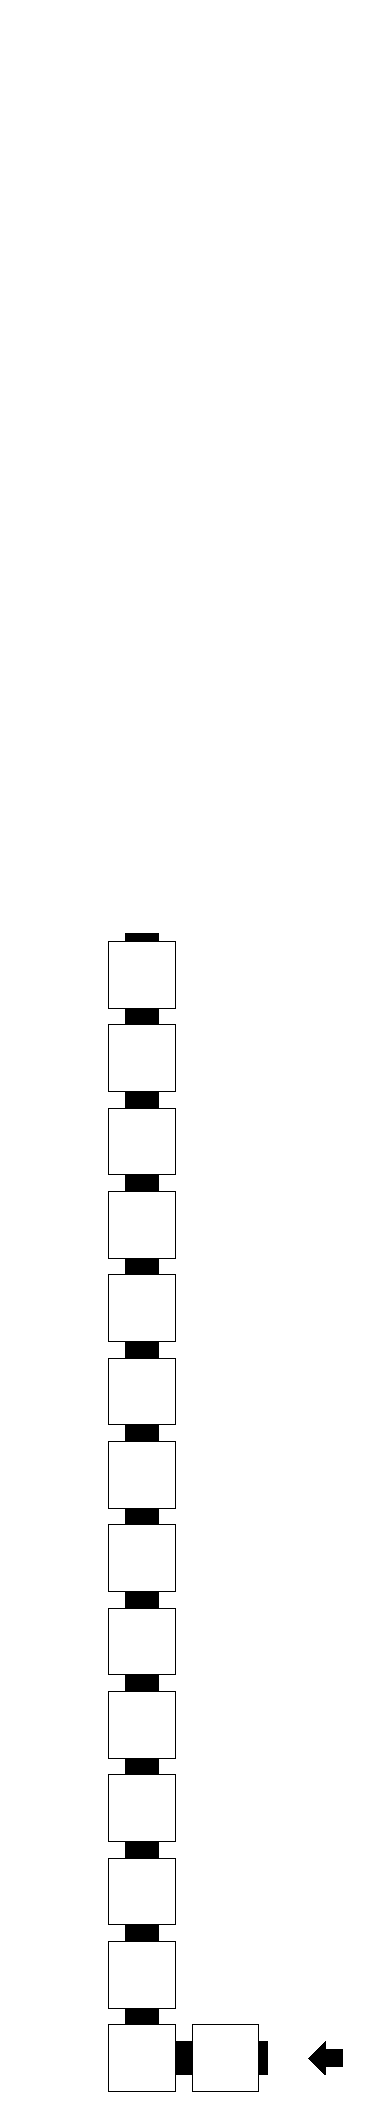
\includegraphics[width=0.2\textwidth]{warping/warp_bridge_case2_digit2_msr}
                \caption{\label{fig:warp_bridge_case2_digit2_msr} Digit 2 -- Case 2}
            \end{subfigure}%
            ~\caption{\label{fig:warp_bridge} {\tt Warp\_Bridge} gadgets}
        \end{figure}




        \item
        Create
        $\begin{aligned}[t]
            \secondwarp(& \left\langle {\tt SecondWarp}, i, u, \inc \right\rangle, \\
                        & \left\langle {\tt SecondWarp}, i, u, \inc \right\rangle, \\
                        & \left\langle {\tt PostWarp},   i, u, \inc \right\rangle \;)
        \end{aligned}$


        \item
        Create
        $\begin{aligned}[t]
            \postwarp(& \left \langle {\tt PostWarp},    i, u, \inc \right\rangle, \\
                      & \left \langle {\tt DigitWriter}, i, u, \inc \right\rangle \;)
        \end{aligned}$

        \begin{figure}[H]
            \begin{subfigure}[t]{0.2\textwidth}
                \centering
                \includegraphics[width=0.2\textwidth]{warping/post_warp_general_digit1}
                \caption{\label{fig:post_warp_general_digit1} General Digit 1}
            \end{subfigure}%
            ~
            \begin{subfigure}[t]{0.2\textwidth}
                \centering
                \includegraphics[width=0.2\textwidth]{warping/post_warp_general_digit2and3}
                \caption{\label{fig:post_warp_general_digit2and3} General Digits 2 and 3 }
            \end{subfigure}%
            ~
            \begin{subfigure}[t]{0.2\textwidth}
                \centering
                \includegraphics[width=0.2\textwidth]{warping/post_warp_case1_digit1_msr}
                \caption{\label{fig:post_warp_case1_digit1_msr} Digit 1 -- Case 1}
            \end{subfigure}%
            ~
            \begin{subfigure}[t]{0.2\textwidth}
                \centering
                \includegraphics[width=0.2\textwidth]{warping/post_warp_case2_digit1_msr}
                \caption{\label{fig:post_warp_case2_digit1_msr} Digit 1 -- Case 2}
            \end{subfigure}%
            ~

            \begin{subfigure}[t]{0.2\textwidth}
                \centering
                \includegraphics[width=0.2\textwidth]{warping/post_warp_case2_digit2_msr}
                \caption{\label{fig:post_warp_case2_digit2_msr} Digit 2 -- Case 2}
            \end{subfigure}%
            ~
            \caption{\label{fig:post_warp_gadgets} {\postwarp} gadgets }
        \end{figure}

    \end{itemize}

    % For each digit length L
\subsubsection{ Digit writers }
% For each index in 1, 2, 3, and carry in 0,1

\begin{itemize}


    \item For each $i = 1,2,3$,
                   $j = l-1,\ldots,1$,
                   $u \in \{0, 1\}^j$, and each
                   $\inc \in \{{\tt increment}, {\tt copy} \}$:
        \begin{itemize}
        \item Create
        $\begin{aligned}[t]
            \dwriter(& \left\langle {\tt Write}, i, u0, \inc \right\rangle,
                       \left\langle {\tt Write}, i, u,  \inc \right\rangle \;)
        \end{aligned}$ \\ from the general gadget in Figure~\ref{fig:write_0}

        \item Create
        $\begin{aligned}[t]
            \dwriter(& \left\langle {\tt Write}, i,  u1, \inc \right\rangle,
                       \left\langle {\tt Write}, i,  u,  \inc \right\rangle \;)
        \end{aligned}$ \\ from the general gadget in Figure~\ref{fig:write_1}


        \item Create
        $\begin{aligned}[t]
            \dwriter(& \left\langle {\tt Write}, 1, u0, \inc, {\tt msr} \right\rangle,
                       \left\langle {\tt Write}, 1, u,  \inc, {\tt msr} \right\rangle \;)
        \end{aligned}$ \\ from the general gadget in Figure~\ref{fig:write_0}

        \item Create
        $\begin{aligned}[t]
            \dwriter(& \left\langle {\tt Write}, 1,  u1, \inc, {\tt msr} \right\rangle,
                       \left\langle {\tt Write}, 1,  u,  \inc, {\tt msr} \right\rangle \;)
        \end{aligned}$ \\ from the general gadget in Figure~\ref{fig:write_1}

        \item Create
        $\begin{aligned}[t]
            \dwriter(& \left\langle {\tt Write}, i, u0, \inc, {\tt msr}, {\tt msd} \right\rangle,
                       \left\langle {\tt Write}, i, u,  \inc, {\tt msr}, {\tt msd} \right\rangle \;)
        \end{aligned}$ \\ from the general gadget in Figure~\ref{fig:write_0}

        \item Create
        $\begin{aligned}[t]
            \dwriter(& \left\langle {\tt Write}, i,  u1, \inc, {\tt msr}, {\tt msd}\right\rangle,
                       \left\langle {\tt Write}, i,  u,  \inc, {\tt msr}, {\tt msd}\right\rangle \;)
        \end{aligned}$ \\ from the general gadget in Figure~\ref{fig:write_1}
        \end{itemize}

    \item For each $i = 1,2,3$ and each $\inc \in \{{\tt increment}, {\tt copy} \}$:
    \begin{itemize}
        \item Create
        $\begin{aligned}[t]
            \dwriter(& \left\langle {\tt Write},    i, 0, \inc \right\rangle,
                       \left\langle {\tt DigitTop}, i,    \inc \right\rangle \;)
        \end{aligned}$ \\ from the general gadget in Figure~\ref{fig:write_0}

        \item Create
        $\begin{aligned}[t]
            \dwriter(& \left\langle {\tt Write},    i, 1, \inc \right\rangle,
                       \left\langle {\tt DigitTop}, i,    \inc \right\rangle \;)
        \end{aligned}$ \\ from the general gadget in Figure~\ref{fig:write_1}

        \item Create
        $\begin{aligned}[t]
            \dwriter(& \left\langle {\tt Write},    1, 0, \inc, {\tt msr} \right\rangle,
                       \left\langle {\tt DigitTop}, 1,    \inc, {\tt msr} \right\rangle \;)
        \end{aligned}$ \\ from the general gadget in Figure~\ref{fig:write_0}

        \item Create
        $\begin{aligned}[t]
            \dwriter(& \left\langle {\tt Write},    1, 1, \inc, {\tt msr} \right\rangle,
                       \left\langle {\tt DigitTop}, 1,    \inc, {\tt msr} \right\rangle \;)
        \end{aligned}$ \\ from the general gadget in Figure~\ref{fig:write_1}

        \item Create
        $\begin{aligned}[t]
            \dwriter(& \left\langle {\tt Write},    i, 0, \inc, {\tt msr}, {\tt msd}\right\rangle,
                       \left\langle {\tt DigitTop}, i,    \inc, {\tt msr}, {\tt msd}\right\rangle \;)
        \end{aligned}$ \\ from the general gadget in Figure~\ref{fig:write_0}

        \item Create
        $\begin{aligned}[t]
            \dwriter(& \left\langle {\tt Write},    i, 1, \inc, {\tt msr}, {\tt msd}\right\rangle,
                       \left\langle {\tt DigitTop}, i,    \inc, {\tt msr}, {\tt msd}\right\rangle \;)
        \end{aligned}$ \\ from the general gadget in Figure~\ref{fig:write_1}
    \end{itemize}


\end{itemize}

\vspace{.5cm}

\begin{figure}[H]
    \centering
    \begin{subfigure}[t]{0.2\textwidth}
        \centering
        \includegraphics[width=0.2\textwidth]{write/write_0}
        \caption{\label{fig:write_0} {\tt Write\_0}}
    \end{subfigure}%
    ~
    \begin{subfigure}[t]{0.2\textwidth}
        \centering
        \includegraphics[width=0.2\textwidth]{write/write_1}
        \caption{\label{fig:write_1} {\tt Write\_1}}
    \end{subfigure}%
    \caption{\label{fig:digit_write} {\tt Digit\_Write} gadgets}
\end{figure}
    \subsubsection{\dtop}

The {\dtop} gadgets have special geometry designed so that {\firstwarp} and
{\secondwarp} tiles are allowed to ``wake up", and complete their warping journey. Each
digit has some type of {\dtop} gadget, however, depending on the digit region
and index of a specific digit, the exact digit top will differ.

% talk about geometry of digit tops enabling first and second warp tiles to "wake up"

\vspace{.5cm}


\begin{figure}[H]
    \centering
    \begin{subfigure}[t]{0.32\textwidth}
        \centering
        \includegraphics[width=0.32\textwidth]{digit_top_general_topper}
        \caption{\label{fig:topper_gen} General topper}
    \end{subfigure}%
    ~
    \begin{subfigure}[t]{0.32\textwidth}
        \centering
        \includegraphics[width=0.32\textwidth]{digit_top_case1_digit1_topper}
        \caption{\label{fig:topper_case1} Case 1 -- topper}
    \end{subfigure}%
    ~
    \begin{subfigure}[t]{0.32\textwidth}
        \centering
        \includegraphics[width=0.32\textwidth]{digit_top_case2_digit2_topper}
        \caption{\label{fig:topper_case2} Case 2 -- topper}
    \end{subfigure}%
    \caption{\label{fig:topper_microgadgets} Topper micro-gadgets }
\end{figure}


For each $\inc \in \{ {\tt increment, copy } \}$
    \begin{itemize}

        \item Digit 1 (general): the following statements create the gadget shown in Figure~\ref{fig:digit_top_general}
        \begin{itemize}
            \item Create
            $\begin{aligned}[t]
                {\tt North\_Line5}(& \left \langle {\tt DigitTop},  1, \inc \right\rangle,
                                     \left \langle {\tt DigitTopA}, 1, \inc \right\rangle \;)
            \end{aligned}$\\from the micro-gadget shown in Figure~\ref{fig:north_line}.

            \item Create
            $\begin{aligned}[t]
                {\tt Topper}(& \left \langle {\tt DigitTopA}, 1, \inc \right\rangle,
                               \left \langle {\tt DigitTopB}, 1, \inc \right\rangle \;)
            \end{aligned}$\\from the micro-gadget shown in Figure~\ref{fig:topper_gen}.

            \item Create
            $\begin{aligned}[t]
                {\tt South\_Line4\textit{l}}(& \left\langle {\tt DigitTopB}, 1, \inc \right\rangle,
                                               \left\langle \returnpath,     1, \inc \right\rangle \;)
            \end{aligned}$\\from the micro-gadget shown in Figure~\ref{fig:south_line}.
        \end{itemize}
        \vspace{1cm}

        \item Digit 1 (MSR): the following statements create the gadget shown in Figure~\ref{fig:digit_top_1_op_msr}
        \begin{itemize}
            \item Create
            $\begin{aligned}[t]
                {\tt Topper}(& \left\langle {\tt DigitTop},  1, \inc, {\tt msr} \right\rangle,
                               \left\langle {\tt DigitTopA}, 1, \inc, {\tt msr} \right\rangle \;)
            \end{aligned}$ \\ from the micro-gadget shown in Figure~\ref{fig:topper_case1}.


            \item Create
            $\begin{aligned}[t]
                {\tt South\_Line4\textit{l}}(& \left\langle {\tt DigitTopA}, 1, \inc, {\tt msr}\right\rangle,
                                               \left\langle \returnpath,     1, \inc, {\tt msr}\right\rangle \;)
            \end{aligned}$ \\ from the micro-gadget shown in Figure~\ref{fig:south_line}.
        \end{itemize}
        \vspace{1cm}


        \item Digit 1 (MSD): the following statements create the gadget shown in Figure~\ref{fig:digit_top_1_op_msr_msd}
        \begin{itemize}
            \item Create
            $\begin{aligned}[t]
                {\tt North\_Line4\textit{l}}(& \left\langle {\tt DigitTop},  1, \inc, {\tt msr}, {\tt msd}\right\rangle,
                                               \left\langle {\tt DigitTopA}, 1, \inc, {\tt msr}, {\tt msd}\right\rangle \;)
            \end{aligned}$\\from the micro-gadget shown in Figure~\ref{fig:north_line}.

            \item Create $\begin{aligned}[t]
                {\tt North\_Line4}(& \left\langle {\tt DigitTopA}, 1, \inc, {\tt msr}, {\tt msd}\right\rangle,
                                     \left\langle {\tt DigitTopB}, 1, \inc, {\tt msr}, {\tt msd}\right\rangle \;)
            \end{aligned}$\\from the micro-gadget shown in Figure~\ref{fig:north_line}.

            \item Create $\begin{aligned}[t]
                {\tt Topper}(& \left\langle {\tt DigitTopB}, 1, \inc, {\tt msr}, {\tt msd}\right\rangle,
                               \left\langle {\tt DigitTopC}, 1, \inc, {\tt msr}, {\tt msd}\right\rangle \;)
            \end{aligned}$\\from the micro-gadget shown in Figure~\ref{fig:topper_gen}.

            \item Create
            $\begin{aligned}[t]
                {\tt South\_Line4\textit{l}}(& \left\langle {\tt DigitTopC}, 1, \inc, {\tt msr}, {\tt msd}\right\rangle,
                                               \left\langle {\tt DigitTopD}, 1, \inc, {\tt msr}, {\tt msd}\right\rangle \;)
            \end{aligned}$\\from the micro-gadget shown in Figure~\ref{fig:south_line}.

            \item Create
            $\begin{aligned}[t]
                {\tt South\_Line30}(& \left\langle {\tt DigitTopD}, 1, \inc, {\tt msr}, {\tt msd}\right\rangle,
                                      \left\langle {\tt DigitTopE}, 1, \inc, {\tt msr}, {\tt msd}\right\rangle \;)
            \end{aligned}$\\from the micro-gadget shown in Figure~\ref{fig:south_line}.

            \item Create
            $\begin{aligned}[t]
                {\tt South\_Line4\textit{l}}(& \left\langle {\tt DigitTopE}, 1, \inc, {\tt msr}, {\tt msd}\right\rangle,
                                               \left\langle {\tt DigitTopF}, 1, \inc, {\tt msr}, {\tt msd}\right\rangle \;)
            \end{aligned}$\\ from the micro-gadget shown in Figure~\ref{fig:south_line}.

            \item Create
            $\begin{aligned}[t]
                {\tt South\_Line14}(& \left\langle {\tt DigitTopF}, 1, \inc, {\tt msr}, {\tt msd}\right\rangle,
                                      \left\langle {\tt DigitTopG}, 1, \inc, {\tt msr}, {\tt msd}\right\rangle \;)
            \end{aligned}$\\ from the micro-gadget shown in Figure~\ref{fig:south_line}.

            \item Create
            $\begin{aligned}[t]
                {\tt South\_Line17}(& \left\langle {\tt DigitTopG}, 1, \inc, {\tt msr}, {\tt msd} \right\rangle,
                                      \left\langle \returnpath,     1, \inc, {\tt msr}, {\tt msd} \right\rangle \;)
            \end{aligned}$\\from the micro-gadget shown in Figure~\ref{fig:south_line}.
        \end{itemize}
        \vspace{1cm}


        \item Digit 2 (general): the following statements create the gadget shown in Figure~\ref{fig:digit_top_general}
        \begin{itemize}
            \item Create
            $\begin{aligned}[t]
                {\tt North\_Line5}(& \left\langle {\tt DigitTop}, 2, \inc \right\rangle,
                                     \left\langle {\tt DigitTopA} 2, \inc \right\rangle \;)
            \end{aligned}$\\from the micro-gadget shown in Figure~\ref{fig:north_line}.

            \item Create
            $\begin{aligned}[t]
                {\tt Topper}(& \left\langle {\tt DigitTopA} 2, \inc \right\rangle,
                               \left\langle {\tt DigitTopB} 2, \inc \right\rangle \;)
            \end{aligned}$\\from the micro-gadget shown in Figure~\ref{fig:topper_gen}.

            \item Create
            $\begin{aligned}[t]
                {\tt South\_Line4\textit{l}}(& \left\langle {\tt DigitTopB} 2, \inc \right\rangle,
                                               \left\langle \returnpath,    2, \inc \right\rangle \;)
            \end{aligned}$\\from the micro-gadget shown in Figure~\ref{fig:south_line}.
        \end{itemize}
        \vspace{1cm}


        \item Digit 2 (MSD): the following statements create the gadget shown in Figure~\ref{fig:digit_top_2_op_msr_msd}
        \begin{itemize}
            \item Create
            $\begin{aligned}[t]
                {\tt North\_Line4\textit{l}}(& \left\langle {\tt DigitTop},  2, \inc, {\tt msr}, {\tt msd} \right\rangle,
                                               \left\langle {\tt DigitTopA}, 2, \inc, {\tt msr}, {\tt msd} \right\rangle\;)
            \end{aligned}$\\ from the micro-gadget shown in Figure~\ref{fig:north_line}.

            \item Create
            $\begin{aligned}[t]
                {\tt Topper}(& \left\langle {\tt DigitTopA}, 2, \inc, {\tt msr}, {\tt msd} \right\rangle,
                               \left\langle {\tt DigitTopB}, 2, \inc, {\tt msr}, {\tt msd} \right\rangle \;)
            \end{aligned}$\\from the micro-gadget shown in Figure~\ref{fig:topper_case2}.

            \item Create
            $\begin{aligned}[t]
                {\tt South\_Line4\textit{l}}(& \left\langle {\tt DigitTopB}, 2, \inc, {\tt msr}, {\tt msd} \right\rangle,
                                               \left\langle {\tt DigitTopC}, 2, \inc, {\tt msr}, {\tt msd} \right\rangle \;)
            \end{aligned}$\\from the micro-gadget shown in Figure~\ref{fig:south_line}.

            \item Create
            $\begin{aligned}[t]
                {\tt South\_Line30}(& \left\langle {\tt DigitTopC}, 2, \inc, {\tt msr}, {\tt msd} \right\rangle,
                                      \left\langle \returnpath,     2, \inc, {\tt msr}, {\tt msd}\right\rangle \;)
            \end{aligned}$\\from the micro-gadget shown in Figure~\ref{fig:south_line}.
        \end{itemize}
        \vspace{1cm}


        \item Digit 3 (general): the following statements create the gadget from Figure~\ref{fig:digit_top_general}
        \begin{itemize}
            \item Create
            $\begin{aligned}[t]
                {\tt North\_Line5}(& \left\langle {\tt DigitTop},  3, \inc \right\rangle,
                                     \left\langle {\tt DigitTopA}, 3, \inc \right\rangle \;)
            \end{aligned}$\\from the micro-gadget shown in Figure~\ref{fig:north_line}.

            \item Create
            $\begin{aligned}[t]
                {\tt Topper}(& \left\langle {\tt DigitTopA}, 3, \inc  \right\rangle,
                               \left\langle {\tt DigitTopB}, 3, \inc  \right\rangle \;)
            \end{aligned}$\\from the micro-gadget shown in Figure~\ref{fig:topper_gen}.

            \item Create
            $\begin{aligned}[t]
                {\tt South\_Line4\textit{l}}(& \left\langle {\tt DigitTopB}, 3, \inc \right\rangle,
                                               \left\langle \returnpath,     3, \inc \right\rangle \;)
            \end{aligned}$\\from the micro-gadget shown in Figure~\ref{fig:south_line}.
        \end{itemize}
        \vspace{1cm}


        \item Digit 3 (MSD): the following statements create the gadget from Figure~\ref{fig:digit_top_general}
        \begin{itemize}
            \item Create
            $\begin{aligned}[t]
                {\tt North\_Line5}(& \left\langle {\tt DigitTop},  3, \inc, {\tt msr}, {\tt msd}\right\rangle,
                                     \left\langle {\tt DigitTopA}, 3, \inc, {\tt msr}, {\tt msd}\right\rangle \;)
            \end{aligned}$\\from the micro-gadget shown in Figure~\ref{fig:north_line}.

            \item Create
            $\begin{aligned}[t]
                {\tt Topper}(& \left\langle {\tt DigitTopA}, 3, \inc, {\tt msr}, {\tt msd}\right\rangle,
                               \left\langle {\tt DigitTopB}, 3, \inc, {\tt msr}, {\tt msd}\right\rangle \;)
            \end{aligned}$\\ from the micro-gadget shown in Figure~\ref{fig:topper_gen}.


            \item Create
            $\begin{aligned}[t]
                {\tt South\_Line4\textit{l}}(& \left\langle {\tt DigitTopB}, 3, \inc, {\tt msr}, {\tt msd}\right\rangle,
                                               \left\langle \returnpath,     3, \inc, {\tt msr}, {\tt msd}\right\rangle \;)
            \end{aligned}$\\ from the micro-gadget shown in Figure~\ref{fig:south_line}.
        \end{itemize}

    \end{itemize}

    \begin{figure}[H]
        \centering
        \subcaptionbox{
            Digits 1, 2, \& 3 - general.
            \label{fig:digit_top_general}
        }{\makebox[0.24\textwidth][c]{\includegraphics[width=0.45in]{digit_top_general}}}%
        ~
        \subcaptionbox{
            Digit 1 - general\\ overview.
            The black tiles in this figure correspond to the gadget shown in subfigure~\subref{fig:digit_top_general}.
            \label{fig:digit_top_1_op_overview}
        }{\makebox[0.24\textwidth][c]{\includegraphics[width=0.45in]{overviews/general/digit_top_1_op}}}%
        ~
        \subcaptionbox{
            Digit 1 - general (seed) overview.
            The black tiles in this figure correspond to the gadget shown in subfigure~\subref{fig:digit_top_general}.
            \label{fig:digit_top_1_seed_op_overview}
        }{\makebox[0.24\textwidth][c]{\includegraphics[width=0.45in]{overviews/general/digit_top_1_seed_op}}}%
        ~
        \subcaptionbox{
            Digit 2 - general\\ overview.
            The black tiles in this figure correspond to the gadget shown in subfigure~\subref{fig:digit_top_general}.
            \label{fig:digit_top_2_op_overview}
        }{\makebox[0.24\textwidth][c]{\includegraphics[width=0.45in]{overviews/general/digit_top_2_op}}}%
        ~
    \end{figure}
    \begin{figure}[H]\ContinuedFloat
        \centering
        \subcaptionbox{
            Digit 2 - general (seed) overview.
            The black tiles in this figure correspond to the gadget shown in subfigure~\subref{fig:digit_top_general}.
            \label{fig:digit_top_2_seed_op_overview}
        }{\makebox[0.24\textwidth][c]{\includegraphics[width=0.45in]{overviews/general/digit_top_2_seed_op}}}%
        ~
        \subcaptionbox{
            Digit 3 - general\\ overview.
            The black tiles in this figure correspond to the gadget shown in subfigure~\subref{fig:digit_top_general}.
            \label{fig:digit_top_3_op_overview}
        }{\makebox[0.24\textwidth][c]{\includegraphics[width=0.45in]{overviews/general/digit_top_3_op}}}%
        ~
        \subcaptionbox{
            Digit 3 - general (seed) overview.
            The black tiles in this figure correspond to the gadget shown in subfigure~\subref{fig:digit_top_general}.
            \label{fig:digit_top_3_seed_op_overview}
        }{\makebox[0.24\textwidth][c]{\includegraphics[width=0.45in]{overviews/general/digit_top_3_seed_op}}}%
        ~
        \subcaptionbox{
            Digit 1 - case 1.
            \label{fig:digit_top_1_op_msr_msd}
        }{\makebox[0.24\textwidth][c]{\includegraphics[width=0.45in]{digit_top_case1_digit1_msr}}}%
        ~
    \end{figure}
    \begin{figure}[H]\ContinuedFloat
        \centering
        \subcaptionbox{
            Digit 1 - case 1 overview.
            The black tiles in this figure correspond to the gadget shown in subfigure~\subref{fig:digit_top_1_op_msr_msd}.
            \label{fig:digit_top_1_op_msr_msd_overview}
        }{\makebox[0.24\textwidth][c]{\includegraphics[width=0.45in]{overviews/case1/digit_top_1_op_msr_msd}}}%
        ~
        \subcaptionbox{
            Digit 1 - case 1 (seed) overview.
            The black tiles in this figure correspond to the gadget shown in subfigure~\subref{fig:digit_top_1_op_msr_msd}.
            \label{fig:digit_top_1_seed_op_msr_msd_overview}
        }{\makebox[0.24\textwidth][c]{\includegraphics[width=0.45in]{overviews/case1/digit_top_1_seed_op_msr_msd}}}%
        ~
        \subcaptionbox{
            Digit 1 - case 2.
            \label{fig:digit_top_1_op_msr}
        }{\makebox[0.24\textwidth][c]{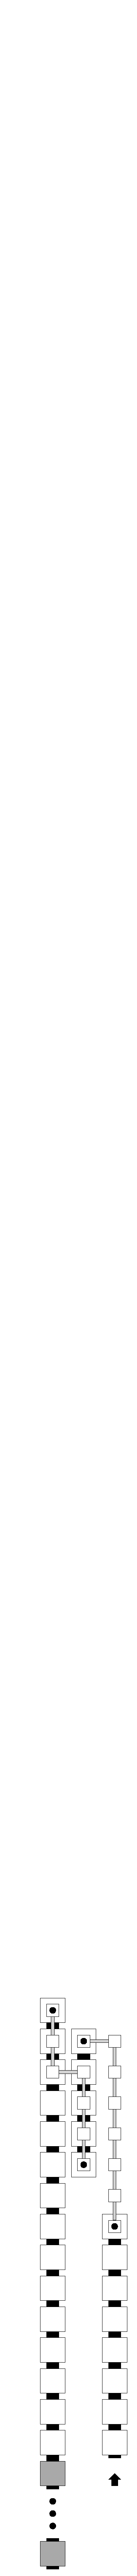
\includegraphics[width=0.45in]{digit_top_case2_digit1_msr}}}%
        ~
        \subcaptionbox{
            Digit 1 - case 2 overview.
            The black tiles in this figure correspond to the gadget shown in subfigure~\subref{fig:digit_top_1_op_msr}.
            \label{fig:digit_top_1_op_msr_overview}
        }{\makebox[0.24\textwidth][c]{\includegraphics[width=0.45in]{overviews/case2/digit_top_1_op_msr}}}%
        ~
    \end{figure}
    \begin{figure}[H]\ContinuedFloat
        \centering
        \subcaptionbox{
            Digit 1 - case 2 (seed) overview.
            The black tiles in this figure correspond to the gadget shown in subfigure~\subref{fig:digit_top_1_op_msr}.
            \label{fig:digit_top_1_seed_op_msr_overview}
        }{\makebox[0.24\textwidth][c]{\includegraphics[width=0.45in]{overviews/case2/digit_top_1_seed_op_msr}}}%
        ~
        \subcaptionbox{
            Digit 2 - case 2.
            \label{fig:digit_top_2_op_msr_msd}
        }{\makebox[0.24\textwidth][c]{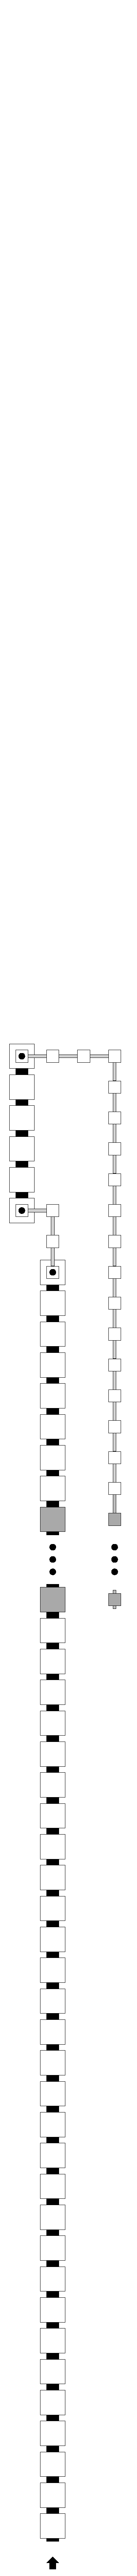
\includegraphics[width=0.45in]{digit_top_case2_digit2_msr}}}%
        ~
        \subcaptionbox{
            Digit 2 - case 2 overview.
            The black tiles in this figure correspond to the gadget shown in subfigure~\subref{fig:digit_top_2_op_msr_msd}.
            \label{fig:digit_top_2_op_msr_msd_overview}
        }{\makebox[0.24\textwidth][c]{\includegraphics[width=0.45in]{overviews/case2/digit_top_2_op_msr_msd}}}%
        ~
        \subcaptionbox{
            Digit 2 - case 2 (seed) overview.
            The black tiles in this figure correspond to the gadget shown in subfigure~\subref{fig:digit_top_2_op_msr_msd}.
            \label{fig:digit_top_2_seed_op_msr_msd_overview}
        }{\makebox[0.24\textwidth][c]{\includegraphics[width=0.45in]{overviews/case2/digit_top_2_seed_op_msr_msd}}}%
        ~
    \end{figure}
    \begin{figure}[H]\ContinuedFloat
        \centering
        \subcaptionbox{
            Digit 3 - case 3.
            \label{fig:digit_top_3_op_msr_msd}
        }{\makebox[0.24\textwidth][c]{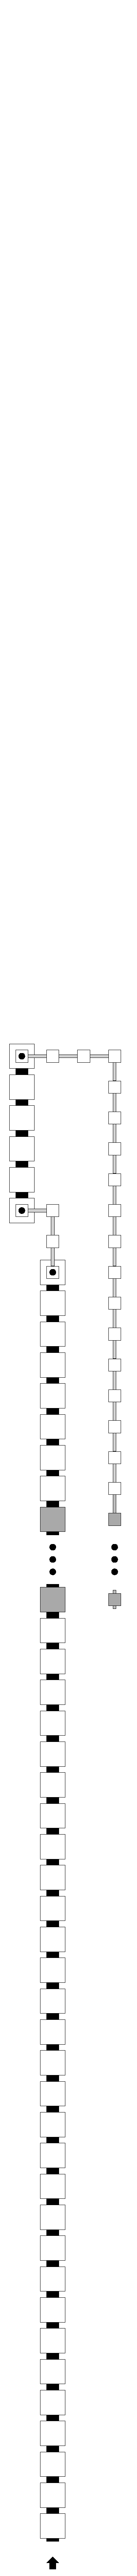
\includegraphics[width=0.33in]{digit_top_case2_digit2_msr}}}%
        ~
        \subcaptionbox{
            Digit 3 - case 3 overview.
            The black tiles in this figure correspond to the gadget shown in subfigure~\subref{fig:digit_top_3_op_msr_msd}.
            \label{fig:digit_top_3_op_msr_msd_overview}
        }{\makebox[0.24\textwidth][c]{\includegraphics[width=0.45in]{overviews/case3/digit_top_3_op_msr_msd}}}%
        ~
        \subcaptionbox{
            Digit 3 - case 3 (seed) overview.
            The black tiles in this figure correspond to the gadget shown in subfigure~\subref{fig:digit_top_3_op_msr_msd}.
            \label{fig:digit_top_3_seed_op_msr_msd_overview}
        }{\makebox[0.24\textwidth][c]{\includegraphics[width=0.45in]{overviews/case3/digit_top_3_seed_op_msr_msd}}}%
        ~
        \caption{\label{fig:digit_tops} The {\tt Digit\_Top} gadgets.}
    \end{figure}

\vspace{1cm}

    \subsubsection{Return paths between digits in the same row}
The gadgets of this class hold a increment/copy signal and the regional index
of the next digit to read. The height of these gadgets is dependent on $l$.
These gadgets are used so that upon writing a digit, the counter
is able to move back down to the next digit in the current row, and continue
reading.
\vspace{1cm}

\begin{figure}[H]
    \centering
    \begin{subfigure}[t]{0.2\textwidth}
        \centering
        \includegraphics[width=0.2\textwidth]{return_paths/return_digit1_read_digit2_general}
        \caption{\label{fig:return_digit1_read_digit2_general} Return digit 1 read digit 2}
    \end{subfigure}%
    ~
    \begin{subfigure}[t]{0.2\textwidth}
        \centering
        \includegraphics[width=0.2\textwidth]{return_paths/return_digit1_read_digit2_case2_msr}
        \caption{\label{fig:return_digit1_read_digit2_case2_msr} Return digit 1 read digit 2 -- Case 2}
    \end{subfigure}%
    ~
    \begin{subfigure}[t]{0.2\textwidth}
        \centering
        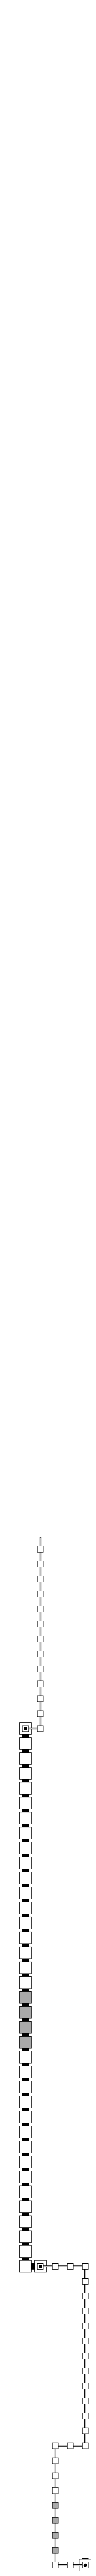
\includegraphics[width=0.2\textwidth]{return_paths/return_digit2_read_digit3_general}
        \caption{\label{fig:return_digit2_read_digit3_general} Return digit 2 read digit 3}
    \end{subfigure}%
    ~
    \begin{subfigure}[t]{0.2\textwidth}
        \centering
        \includegraphics[width=0.2\textwidth]{return_paths/return_digit3_read_digit1_general}
        \caption{\label{fig:return_digit3_read_digit1_general} Return digit 3 read digit 1}
    \end{subfigure}%
    \caption{\label{fig:return_path_same_row} All of these gadgets grow from north to south, the height of gray tiles depends on $l$.}
\end{figure}

\noindent For each {\inc} $\in \{ {\tt increment, copy } \}$.

% todo yes/no?: pass L as input since gadget size is O(L), but inputs/outputs don't depend on it

\begin{itemize}
    \item Create
    $\begin{aligned}[t]
        \returnfromdonereaddtwo(& \left \langle {\tt ReturnD1ReadD2},          \inc \right\rangle, \\
                                & \left \langle {\tt DigitReader}, 2, \lambda, \inc \right\rangle \;)
    \end{aligned}$

    \item Create
    $\begin{aligned}[t]
        \returnfromdonereaddtwocasetwo(& \left \langle {\tt ReturnD1ReadD2-Case2},    \inc \right\rangle, \\
                                        & \left \langle {\tt DigitReader}, 2, \lambda, \inc \right\rangle \;)
    \end{aligned}$

    \item Create
    $\begin{aligned}[t]
        \returnfromdtworeaddthree(& \left \langle {\tt ReturnD2ReadD3},             \inc \right\rangle, \\
                                    & \left \langle {\tt DigitReader},  3, \lambda, \inc \right\rangle \;)
    \end{aligned}$

    \item Create
    $\begin{aligned}[t]
            \returnfromdthreereaddone(& \left \langle {\tt ReturnD3ReadD1},           \inc \right\rangle, \\
                                    & \left \langle {\tt DigitReader},  1, \lambda,   \inc \right\rangle \;)
    \end{aligned}$

\end{itemize}


    \subsubsection{Return paths between the MSD and LSD in different rows}

The gadgets of this class hold a increment/copy signal.
The height of these gadgets is dependent on $l$ and the width is dependent of $k$.
These gadgets are used to begin reading the first digit in the following row, once
the MSD has been read in the current row.
\vspace{1cm}

\begin{figure}[H]
    \centering
    \begin{subfigure}[t]{0.3\textwidth}
        \centering
        \includegraphics[width=0.3\textwidth]{return_paths/return_digit1_read_next_row}
        \caption{\label{fig:return_digit1_read_next_row} Case -- 1}
    \end{subfigure}%
    ~
    \begin{subfigure}[t]{0.3\textwidth}
        \centering
        \includegraphics[width=0.3\textwidth]{return_paths/return_digit2_read_next_row}
        \caption{\label{fig:return_digit2_read_next_row} Case -- 2}
    \end{subfigure}%
    ~
    \begin{subfigure}[t]{0.3\textwidth}
        \centering
        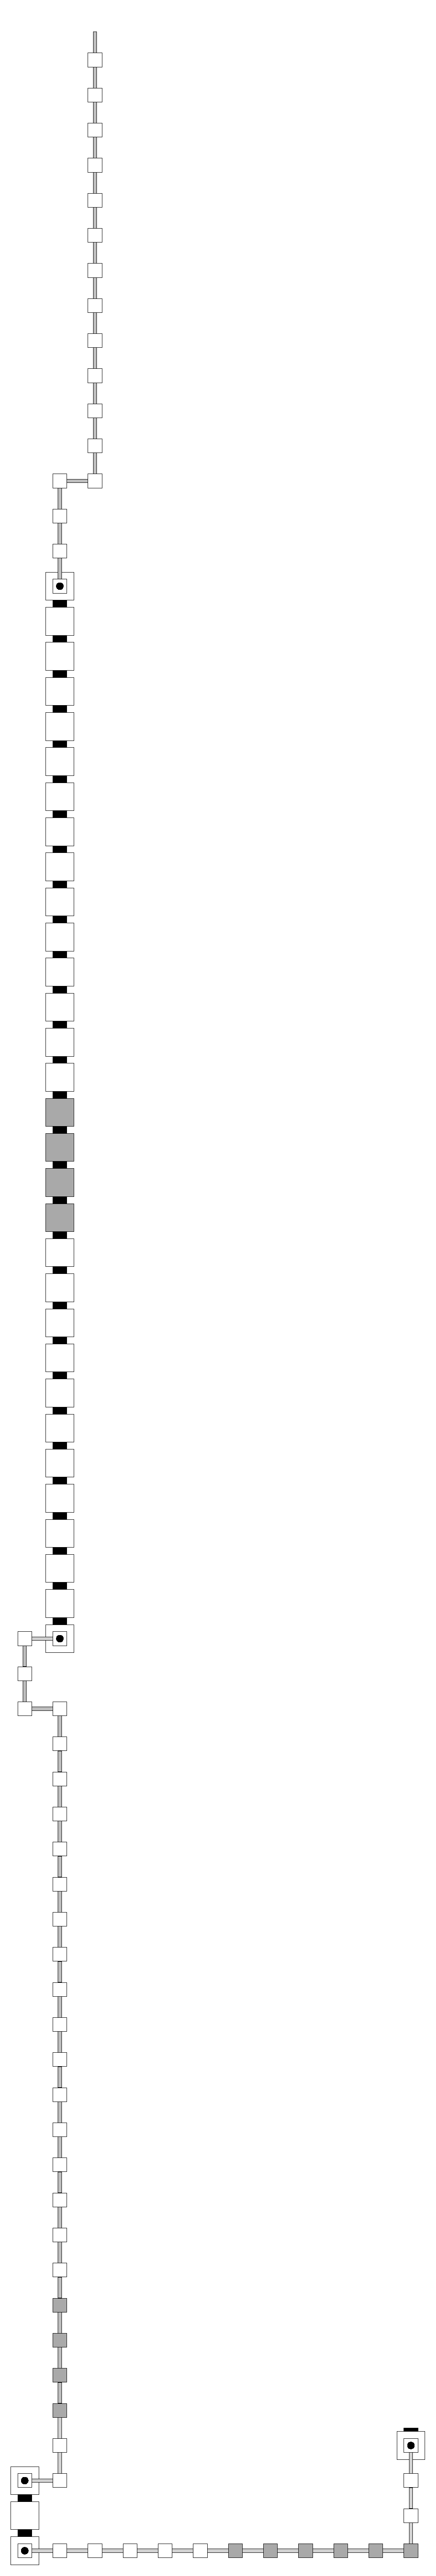
\includegraphics[width=0.3\textwidth]{return_paths/return_digit3_read_next_row}
        \caption{\label{fig:return_digit3_read_next_row} Case -- 3}
    \end{subfigure}%
    \caption{\label{fig:return_path_next_row} {\tt Return\_From\_Digit\_Read\_Next\_Row} gadgets.
    All of these gadgets assemble north to south. The vertical gray lines tiles have a height
    that depends on $l$ and the horizontal gray lines depend on $k$. (cases 1 and 2 are geometrically equivalent)}
\end{figure}

\noindent For each $\inc \in \{  {\tt increment, copy } \}$

\begin{itemize}
    \item Create
    $\begin{aligned}[t]
        \returnfromdonereadnextrow(& \left \langle {\tt ReturnD1ReadNextRow},     \inc \right\rangle,
                                     \left \langle {\tt DigitReader}, 1, \lambda, \inc \right\rangle \;)
    \end{aligned}$
    \\ from the general gadget in Figure~\ref{fig:return_digit1_read_next_row}

    \item Create
    $\begin{aligned}[t]
        \returnfromdtworeadnextrow(& \left \langle {\tt ReturnD2ReadNextRow},     \inc \right\rangle,
                                     \left \langle {\tt DigitReader}, 1, \lambda, \inc \right\rangle \;)
    \end{aligned}$
    \\ from the general gadget in Figure~\ref{fig:return_digit2_read_next_row}

    \item Create
    $\begin{aligned}[t]
        \returnfromdthreereadnextrow(& \left \langle {\tt ReturnD3ReadNextRow},     \inc \right\rangle,
                                       \left \langle {\tt DigitReader}, 1, \lambda, \inc \right\rangle \;)
    \end{aligned}$
    \\ from the general gadget in Figure~\ref{fig:return_digit3_read_next_row}
\end{itemize}

\subsection{Overviews}

\begin{figure}[H]
    \centering
    \begin{subfigure}[t]{0.3\textwidth}
        \centering
        \includegraphics[width=0.3\textwidth]{full_overview_case3_colored}
        \caption{\label{fig:full_overview_case3_colored} Full overview case 3}
    \end{subfigure}%
    ~
    \begin{subfigure}[t]{0.3\textwidth}
        \centering
        \includegraphics[width=0.3\textwidth]{full_overview_case2_colored}
        \caption{\label{fig:full_overview_case2_colored} Full overview case 2}
    \end{subfigure}%
    ~
    \begin{subfigure}[t]{0.3\textwidth}
        \centering
        \includegraphics[width=0.3\textwidth]{full_overview_case1_colored}
        \caption{\label{fig:full_overview_case1_colored} Full overview case 1}
    \end{subfigure}%
    ~
\end{figure}